% arara: pdflatex
% arara: bibtex
% arara: pdflatex
% arara: pdflatex
\documentclass[11pt]{article}



\setlength{\textheight}{225mm}
\setlength{\textwidth}{165mm}
\setlength{\oddsidemargin}{-5mm}
\setlength{\topmargin}{-5mm}

\usepackage{amssymb,amsmath,amsthm}
\usepackage{latexsym,amsfonts}
\usepackage{color}
\usepackage{graphicx}
  \graphicspath{{./Figures/}}
  \DeclareGraphicsExtensions{.jpeg,.png,.jpg,.eps,.pdf}
\usepackage{tikz}
\usepackage{epstopdf}
\usepackage{hyperref}
\usepackage{xcolor}
\newcommand{\stirlingii}{\genfrac{\{}{\}}{0pt}{}}

\usepackage{natbib}
\usepackage[T1]{fontenc} % Font encoding
\usepackage{times} % Times New Roman font
\usepackage{comment}
\usepackage{bbm}
\usepackage{cancel}
% This file contains the notation for the book on hidden Markov processes.
% Latest update on 15.08.09, rearranging, grouping, and getting rid of
% unnecessary definitions.

% Bold face Roman symbols

\def\oneb{{\bf 1}}

\def\a{{\bf a}}
\def\b{{\bf b}}
\def\c{{\bf c}}
\def\dd{{\bf d}}
\def\eb{{\bf e}}
\def\f{{\bf f}}
\def\gbold{{\bf g}}
\def\gb{{\bf g}}
\def\h{{\bf h}}
\def\i{{\bf i}}
\def\j{{\bf j}}
\def\J{{\bf J}}
\def\k{{\bf k}}
\def\p{{\bf p}}
\def\q{{\bf q}}
\def\rbold{{\bf r}}
\def\u{{\bf u}}
\def\v{{\bf v}}
\def\w{{\bf w}}
\def\x{{\bf x}}
\def\y{{\bf y}}
\def\z{{\bf z}}
\def\Z{{\bf Z}}

% Calligraphic symbols

\def\A{{\cal A}}
\def\B{{\cal B}}
\def\C{{\cal C}}
\def\Dcal{{\cal D}}
\def\E{{\cal E}}
\def\F{{\cal F}}
\def\G{{\cal G}}
\def\H{{\cal H}}
\def\I{{\cal I}}
\def\Lcal{{\cal L}}
\def\M{{\cal M}}
\def\N{{\cal N}}
\def\P{{\cal P}}
\def\Q{{\cal Q}}
\def\Rcal{{\cal R}}
\def\S{{\cal S}}
\def\T{{\cal T}}
\def\U{{\cal U}}
\def\V{{\cal V}}
\def\X{{\cal X}}
\def\Y{{\cal Y}}
\def\Zcal{{\cal Z}}

% Blackboard style symbols

\def\Abb{{\mathbb A}}
\def\Bbb{{\mathbb B}}
\def\Cbb{{\mathbb C}}
\def\Fbb{{\mathbb F}}
\def\Mbb{{\mathbb M}}
\def\Nbb{{\mathbb N}}
\def\Nm{{\mathbb N}}
\def\R{{\mathbb R}}
\def\Sbb{{\mathbb S}}
\def\Sm{{\mathbb S}}
\def\Xbb{{\mathbb X}}
\def\Ybb{{\mathbb Y}}
\def\Zbb{{\mathbb Z}}
\def\Zm{{\mathbb Z}}

% Abbreviations for greek letters

\def\al{\alpha}
\def\d{\delta}
\def\D{\Delta}
\def\e{\epsilon}
\def\g{\gamma}
\def\GA{\Gamma}
\def\l{\lambda}
\def\L{\Lambda}
\def\om{\omega}
\def\OM{\Omega}
\def\r{\rho}
\def\s{\sigma}
\def\SI{\Sigma}
\def\t{\tau}
\def\th{\theta}
\def\Th{\Theta}

% Bold greek letters

\def\balpha{{\boldsymbol \alpha}}
\def\bbeta{{\boldsymbol \beta}}
\def\boldeta{{\boldsymbol \eta}}
\def\beps{{\boldsymbol \e}}
\def\bgamma{{\boldsymbol \gamma}}
\def\bl{{\boldsymbol \lambda}}
\def\bmu{{\boldsymbol \mu}}
\def\bnu{{\boldsymbol \nu}}
\def\bom{{\boldsymbol \om}}
\def\bth{{\boldsymbol \theta}}
\def\bphi{{\boldsymbol \phi}}
\def\bpsi{{\boldsymbol \psi}}
\def\bpi{{\boldsymbol \pi}}
\def\bsig{{\boldsymbol \sigma}}
\def\bxi{{\boldsymbol \xi}}
\def\bzeta{{\boldsymbol \zeta}}
\def\bD{\mathbf{\D}}

% Bars, hats, tildes etc.

\def\ab{\bar{a}}
\def\ah{\hat{\a}}
\def\Ab{\bar{A}}
\def\Bb{\bar{\B}}
\def\bmuh{\hat{\bmu}}
\def\ct{\tilde{c}}
\def\cub{\bar{c}}
\def\clb{\underline{c}}
\def\cb{\bar{c}}
\def\db{\bar{d}}
\def\dh{\hat{d}}
\def\Eh{\hat{E}}
\def\fb{\bar{f}}
\def\fh{\hat{f}}
\def\Jb{\bar{J}}
\def\Jh{\hat{J}}
\def\kb{\bar{k}}
\def\Ot{\tilde{O}}
\def\pb{\bar{p}}
\def\ph{\hat{p}}
\def\Pb{\bar{P}}
\def\PB{\bar{\cal P}}
\def\Ph{\hat{P}}
\def\Pt{\tilde{P}}
\def\Ptt{\tilde{\P}}
\def\qb{\bar{q}}
\def\qbh{\hat{\q}}
\def\Qh{\hat{Q}}
\def\Qt{\tilde{Q}}
\def\rbar{\bar{\rho}}
\def\sbold{\mathbf{s}}
\def\Sb{\bar{S}}
\def\ub{\bar{u}}
\def\vb{\bar{v}}
\def\vh{\hat{v}}
\def\Vh{\hat{V}}
\def\xb{\bar{x}}
\def\xt{\tilde{x}}
\def\yb{\bar{y}}
\def\zb{\bar{z}}
\def\zt{\tilde{z}}

\def\alb{\bar{\al}}
\def\lb{\bar{\l}}
\def\nub{\bar{\nu}}
\def\thb{\bar{\theta}}
\def\xib{\bar{\xi}}

\def\muh{\hat{\mu}}

% Approaching infinity

\def\kai{k \ap \infty}
\def\lai{l \ap \infty}
\def\mai{m \ap \infty}
\def\nai{n \ap \infty}
\def\tai{t \ap \infty}
\def\Tai{T \ap \infty}

% Miscellaneous mathematical symbols

\def\ap{\rightarrow}
\def\arg{{\rm arg}}
\def\lip{\langle}
\def\rip{\rangle}
\def\es{\emptyset}
\def\seq{\subseteq}
\def\dag{\dagger}

\def\bi{\{0,1\}}
\def\bim{\bi^m}
\def\bin{\bi^n}
\def\bimn{\bi^{m \times n}}
\def\bino{\bi^{n_r \times n_c}}
\def\bp{\{-1,1\}}
\def\bz{{\bf 0}}
\def\imp{\; \Longrightarrow \;}
\def\orr{\vee}
\def\fa{\; \forall}
\def\mult{x_1 , \ldots , x_m}
\def\xvec{[ x_1 \ldots x_m ]^t}

\def\half{\frac{1}{2}}
\def\ae{\mbox{ a.e.}}
\def\as{\mbox{ a.s.}}
\def\wp{\mbox{ w.p.}}
\def\sg{\mbox{sign}}
\def\st{\mbox{ s.t. }}
\def\nm{\Vert}
\def\mgf{{\rm mgf}}

\renewcommand{\iff}{\mbox{$\; \; \Longleftrightarrow \; \;$}}
\renewcommand{\and}{\mbox{$\wedge$}}

% Typesetting commands

\newcommand{\bc}{\begin{center}}
\newcommand{\ec}{\end{center}}
\newcommand{\be}{\begin{equation}}
\newcommand{\ee}{\end{equation}}
\newcommand{\bd}{\begin{displaymath}}
\newcommand{\ed}{\end{displaymath}}
\newcommand{\ba}{\begin{array}}
\newcommand{\ea}{\end{array}}
\newcommand{\ben}{\begin{enumerate}}
\newcommand{\een}{\end{enumerate}}
\newcommand{\bit}{\begin{itemize}}
\newcommand{\eit}{\end{itemize}}
\newcommand{\beq}{\begin{eqnarray}}
\newcommand{\eeq}{\end{eqnarray}}
\newcommand{\btab}{\begin{tabular}}
\newcommand{\etab}{\end{tabular}}
\newcommand{\bfig}{\begin{figure}}
\newcommand{\efig}{\end{figure}}
\newcommand{\btp}{\begin{tikzpicture}}
\newcommand{\etp}{\end{tikzpicture}}

% Additional commands for compressed sensing papers

\newcommand{\argmin}{\operatornamewithlimits{arg~min}}
\newcommand{\argmax}{\operatornamewithlimits{arg~max}}
\renewcommand{\mod}{~{\rm mod}~}

% \DeclareMathOperator*{\argmin}{arg\,min}
% \DeclareMathOperator*{\argmax}{arg\,max}

\def\boldr{{\bf r}}
\def\cons{{\mbox{const}}}

% Norm symbols

\newcommand{\nmm}[1]{ \nm #1 \nm }
\newcommand{\nmeu}[1]{ \nm #1 \nm_2 }
\newcommand{\nmeusq}[1]{ \nm #1 \nm_2^2 }
\newcommand{\nmi}[1]{ \nm #1 \nm_\infty}
\newcommand{\nmA}[1]{ \nm #1 \nm_A }
\newcommand{\nmF}[1]{ \nm #1 \nm_F }
\newcommand{\nmmax}[1]{ \nm #1 \nm_M }
\newcommand{\nmmnu}[1]{ \nm #1 \nm_\nu }
\newcommand{\nmM}[1]{ \nm #1 \nm_M }
\newcommand{\nmN}[1]{ \nm #1 \nm_N }
\newcommand{\nmP}[1]{ \nm #1 \nm_P }
\newcommand{\nmS}[1]{ \nm #1 \nm_S }
\newcommand{\nmp}[1]{ \nm #1 \nm_p }
\newcommand{\nmq}[1]{ \nm #1 \nm_q }
\newcommand{\nmv}[1]{ \nm #1 \nm_v }
\newcommand{\nmV}[1]{ \nm #1 \nm_V }
\newcommand{\nmcmu}[1]{ \nm #1 \nm_{C,\mu} }
\newcommand{\nmgmu}[1]{ \nm #1 \nm_{{\rm SGL},\mu} }

% Additional commands for stochastic approximation (SA) papers.

\def\gJ{\nabla J}
\def\bths{\bth^*}
\def\bphit{\tilde{\bphi}}
% \def\bphH{\bphi^{HB}_{t+1}}
\def\bphH{\bphi_{t+1}}
\def\bphN{\bphi^{NAG}_{t+1}}
% \def\phH{\bphit^{HB}_t}
\def\phH{\bphit_t}
\def\phN{\bphit^{NAG}_t}


\def\Bb{\bar{B}}
\def\Cb{\bar{C}}
\def\Zb{\bar{Z}}

% Ordinary and partial derivatives symbols.
\newcommand{\dx}[2]{\frac{d#1}{d#2}}
\newcommand{\px}[2]{\frac{\partial #1}{\partial #2}}
\newcommand{\tpx}[3]{\frac{\partial^2 #1}{\partial #2 \partial #3}}

% Quadratic variation symbol
\newcommand{\QV}[1]{ \langle #1 \rangle }

% Inner product symbol
\newcommand{\IP}[2]{ \langle #1 , #2 \rangle }
\newcommand{\IPF}[2]{ \langle #1 , #2 \rangle_F }

% Combinatorial parameter symbol
\newcommand{\nchk}[2]{ \left( \ba{c} #1 \\ #2 \ea \right) }
% Legendre symbol
\newcommand{\Leg}[2]{ \left( \frac{#1}{#2} \right) }

% \newcommand{\halmos}{\hfill $\Box$}
\newcommand{\halmos}{\hfill $\blacksquare$}

% Basis pursuit symbol
\def\DBP{\D_{{\rm BP}}}


% \newcommand{\det}{{\rm det}}
\newcommand{\rk}{{\rm{rank}}}
\newcommand{\supp}{{\rm{supp}}}
\newcommand{\tr}{{\rm{tr}}}
% \newcommand{\mod}{\rm{ mod }}



\def\vcd{\mbox{VC-dim}}
\def\pd{\mbox{P-dim}}

% Compressed Sensing symbols.

\def\Up{U_\perp}
\def\Upt{U_\perp^\top}
\def\Vp{V_\perp}
\def\Vpt{V_\perp^\top}
\def\fnrc{\frac{1}{\alpha}}
\def\fdrc{\al}
\def\foal{(1/\al)}
\def\anr{\alpha\sqrt{n_rn_c}}
\def\anrs{\alpha^2n_rn_c}
\def\fnrcs{\frac{1}{\alpha^2}}
\def\foals{(1/\al^2)}
\def\drc{(d_r,d_c)}

\def\Cm{\Cbb^m}
\def\Cn{\Cbb^n}
\def\Cr{\Cbb^r}
\def\Cs{\Cbb^s}
\def\Ckl{\Cbb^{k \times l}}
\def\Cmn{\Cbb^{m \times n}}
\def\Cmr{\Cbb^{m \times r}}
\def\Cnn{\Cbb^{n \times n}}
\def\Cno{\Cbb^{n_r \times n_c}}
\def\Cns{\Cbb^{n \times s}}
\def\Crr{\Cbb^{r \times r}}
\def\Crs{\Cbb^{r \times s}}
\def\Fm{\Fbb_2^m}
\def\Fmn{\Fbb_2^{m \times n}}
\def\Fn{\Fbb_2^n}
\def\Fp{\Fbb_p}
\def\Fq{\Fbb_q}
\def\Fqs{\Fbb_q^*}
\def\PGq{PGL(2,\Fq)}
\def\PSq{PSL(2,\Fq)}
\def\PScq{PSL^c(2,\Fq)}
\def\Rkl{\R^{k \times l}}
\def\Rmn{\R^{m \times n}}
\def\Rno{\R^{n_r \times n_c}}
\def\Sno{\Sm^{n_r \times n_c}}

\def\ulo{u_{\L_0}}
\def\uloc{u_{\L_0^c}}
\def\vlo{v_{\L_0}}
\def\vloc{v_{\L_0^c}}
\def\xd{x_\downarrow}
\def\xh{\hat{x}}
\def\Xh{\hat{X}}
\def\xl{x_{\L}}
\def\xlc{x_{\L^c}}
\def\xlo{x_{\L_0}}
\def\xloc{x_{\L_0^c}}
\def\hl{h_{\L}}
\def\hlc{h_{\L^c}}
\def\hlo{h_{\L_0}}
\def\hloc{h_{\L_0^c}}
\def\hso{h_{S_0}}
\def\hsoc{h_{S_0^c}}

\def\GkS{{\rm GkS}}
\def\ru{\underline{\r}}
\def\rb{\bar{\r}}



\def\nmsl1{\nm_{{\rm SL1}}}

\usepackage{accents}
\newcommand{\qleq}{\accentset{?}{\leq}}

% Special notation for this paper.

\definecolor{verm}{rgb}{0.6,0.2,0.2}
\definecolor{purp}{rgb}{0.3,0.1,0.6}
\definecolor{purple}{rgb}{0.4,0.0,0.6}
\definecolor{bggreen}{rgb}{0.1,0.3,0.1}
\definecolor{dgreen}{rgb}{0.1,0.6,0.1}
\definecolor{black}{rgb}{0.0,0.0,0.0}
\definecolor{crim}{rgb}{0.3,0.1,0.1}
\definecolor{dred}{rgb}{0.5,0.1,0.1}

\newtheorem{corollary}{Corollary}{\bf}{\it}
\newtheorem{definition}{Definition}{\bf}{\it}
\newtheorem{example}{Example}{\bf}{\rm}
\newtheorem{lemma}{Lemma}{\bf}{\it}	
\newtheorem{theorem}{Theorem}{\bf}{\it}
\newtheorem{proposition}{Proposition}{\bf}{\it}
\newtheorem{conjecture}{Conjecture}{\bf}{\it}
\newtheorem{problem}{Problem}{\bf}{\rm}
\newtheorem{assumption}{Assumption}{\bf}{\it}	
\newcommand{\inlinemath}[1]{\fcolorbox{red}{white}{\ensuremath{#1}}}

\usetikzlibrary{shapes, arrows.meta}
\usetikzlibrary{decorations.pathreplacing}
\usepackage{enumitem,amssymb}
\newlist{todolist}{itemize}{2}
\setlist[todolist]{label=$\square$}
\usepackage{pifont}
\newcommand{\cmark}{\ding{51}}%
\newcommand{\xmark}{\ding{55}}%
\newcommand{\done}{\rlap{$\square$}{\raisebox{2pt}{\large\hspace{1pt}\cmark}}%
\hspace{-2.5pt}}
\newcommand{\wontfix}{\rlap{$\square$}{\large\hspace{1pt}\xmark}}

\usepackage{pgfplots}

\def\W{\mathcal{W}}
\begin{document}

\title{Parsimonious and Structured Learning\\
Introduction to Submodular Optimization}

\author{Uday Kiran Reddy Tadipatri
\thanks{Ph.D Student, Electrical \& Systems Engineering. 
Mail-Id: \href{mailto:ukreddy@seas.upenn.edu}{\textit{ukreddy@seas.upenn.edu}}}}

\date{\today}
\maketitle
This note is an introduction to submodular functions and optimization. The content is highly
inspired by the monologue and slides of
\cite{bach_learning_2013a}, \cite{jan-website-24}.

In the real world, we encounter many discrete optimization problems where the feasible set is discrete,
and there could be a combinatorial number of possible feasible points. In such cases, solving the optimization
problem is computationally intensive, or one would have to settle for approximate solutions offered by 
greedy algorithms. Submodular optimization is a class of combinatorial optimization problems where the objective 
function is submodular. This class of problems has many interesting properties that allow us to translate these 
combinatorial optimization problems into convex optimization problems, enabling us to utilize tools learned in 
convex analysis to solve these problems efficiently.


Submodular functions arise in many applications such as machine learning, computer vision, 
signal processing, and electrical networks. In this note, we will introduce submodular functions, 
Lovász extension, and the connections between submodular and convex optimization. We shall conclude with 
an application to structured sparsity problems in machine learning.

\section{Submodular Functions}
As a notation we denote, $\V$ as finite set, and $2^{\V}$ as the power set of $\V$. Upper-case $F$ denotes
a function acting on the set of $2^{\V}$, lower-case $f$ indicates function acting on real vectors. 
\begin{definition}{Submodular Function:}
A set-function $F: 2^{\V} \to \R$ is submodular if and only if,
for all subsets $\A, \B \subseteq \V$, we have: $F(\A) + F(\B) \geq F(\A \cup \B) + F(\A \cap \B)$.
\end{definition}
We always assume that, $F(\varnothing) = 0$. Note that if function, $F$ is submodular
then it implies sub-additivity, but converse is not true.

There are alternative ways to define 
submodular functions,

\begin{definition}{First-order differences:} The set-function $F: 2^{\V} \to \R$ is submodular if and only if
for all subsets $\A \subseteq \B \subseteq \V$, and $i \in \V \backslash \B$, we have: $F(\A \cup \{i\}) - F(\A) \geq F(\B \cup \{i\}) - F(\B)$.
\end{definition}

\begin{definition}{Second-order differences:} The set-function $F: 2^{\V} \to \R$ is submodular if and only if
for all subsets $\A \subseteq \V$, and $i, j \in \V \backslash \A$, we have: 
$F(\A \cup \{i\}) - F(\A) \geq F(\A \cup \{i, j\}) - F(\A \cup \{j\})$.
\end{definition}

Verify from any of the above definition that the above function is submodular.

\begin{example}[Cardinality]
A simple example of submodular function is the cardinality function, $F(\A) = |\A|$.
This function is also classified as modular function.
\end{example}

\begin{example}[Graph Cut]
Take a graph, $\G$ denote $\V(\G) = \{v_1, \dots, v_n\}$ 
to be set of vertices. The function, $F(\S) = |\{(u, v): (u, v) \in \E(\G) u \in \A, \v \in \V(\G)\backslash \A\}|$,
where, $\S \subseteq \V(\G)$ is submodular.
\end{example}
Verify the above example from First-order differences definition.

\begin{example}[Mutual Information]
Denote, $\Omega = \{X_1, X_2, \dots, X_n\}$ be set of 
random variables. The mutual information between, $\S$ and $\Omega \backslash \S$, where $\S \subseteq \Omega$
is submodular, i.e, $F(\S) = I(\S; \Omega \backslash \S)$.
\end{example}

Verify from the original definition that the above example is submodular.

Similar to the analogy of convex-concave function, we can also define supermodular functions.
If a function is both submodular and supermodular, then it is called modular function. For instance, the earlier 
example is a modular function.

Now we move-on to some operations that preserve submodularity.

\begin{enumerate}
\item \textbf{Extension:} Let $\B \subseteq \V$, then $G: 2^{\B} \to \R$ be a submodular function, then
function $F: 2^{\V} \to \R$ defined as $F(\A) := G(\A \cap \B); \forall \A \subseteq \V$ is also submodular.
\item \textbf{Restriction:} Let $\B \subseteq \V$, then $G: 2^{\V} \to \R$ be a submodular function, then
function $F: 2^{\B} \to \R$ defined as $F(\A) := G(\A); \forall \A \subseteq \B$ is also submodular.
\item \textbf{Contraction:} Let $\B \subseteq \V$, then $G: 2^{\V} \to \R$ be a submodular function, then
the function $F: 2^{\V \backslash \B} \to \R$ defined as $F(\A) := G(\A \cup \B) - G(\B); \forall \A \subseteq \V \backslash \B$ 
is also submodular.
\item \textbf{Partial Minimization:} Take disjoint sets $\V, \W$ and submodular function $G: 2^{\V \cup \W} \to \R$.
Then function $F: 2^{\V} \to \R$ defined as
$F(\A) := \min_{\B \subseteq \W}G(A \cup B) - \min_{B \subseteq \W}G(B)$ is a submodular function.
\item \textbf{Convolution:} 
Let function $F: 2^{\V} \to \R$ be a submodular function, and take a vector $\z \in \R^{p}$.
Then the fucntion $G: 2^{\V} \to \R$ defined as $G(\A) := \min_{\B \subseteq \A}F(\B) + \sum_{i \in \A \backslash \B}z_i$
is a submodular function. Moreover, $G(\A) \leq F(\A)$, $G(\A) \leq \sum_{i \in \A}z_i$.
\item \textbf{Monotonization:} Let $F: 2^{\V} \to \R$ be a submodular function.
Then function $G: 2^{\V} \to \R$ defined as $G(\A) := \min_{\B \supset \A} F(\B) - \min_{\B \subseteq \A}F(\B)$
is submodular. Moreover, $G(\A) \leq F(\A)$.
\end{enumerate}

\section{Lovász Extension: A bridge that connects Submodular Optimization to Convex Optimization}

\begin{definition}Given
a set-function $F: 2^{\V} \to \R$ (not necessarily submodular), the Lovász extension $f: \R^{p} \to \R$ \footnote{$p = |\V|$}
is defined as follows; for $\w \in \R^{p}$, order the components
in decreasing order $w_{j1} \geq w_{j2} \geq \dots \geq w_{jp}$, where $(j1, j2, \dots, jp)$ is arg sort order.
The below definitions are equivalent:
\begin{enumerate}
  \item $f(\w) = \sum_{k=1}^{p}w_{jk}\left[F(\{j1, \dots j{k}\}) - F(\{j1, \dots j{k-1}\})\right]$,
  \item $f(\w) = \sum_{k=1}^{p-1}F(\{j1, \dots, jk\})(w_{jk} - w_{j{k+1}}) + F(\V)w_{jp}$,
  \item $f(\w) = \int_{\min\{w_1, \dots, w_p\}}^{\infty}F(\{\w \geq z\})dz + F(V)\min\{w_1, \dots, w_p\}$
  \item $f(\w) = \int_{0}^{\infty}F(\{\w \geq z\})dz + \int_{-\infty}^{0}\left[F(\{\w \geq z\}) - F(\V)\right]dz$ 
\end{enumerate}
\end{definition}

\begin{example}
Let consider a set function, $F : 2^{\{1, 2\}} \to \R$
such that, $F(\varnothing) = 0, F(\{1\}) = 1, F(\{2\}) = 1, F(\{1, 2\}) = 0$.

The Lovász extension of the above function is as follows:
\bd
f([x_1; x_2]) = \begin{cases}
x_2 - x_1  & \text{ if }x_1 \leq x_2\\
x_1 - x_2 & \text{Otherwise}
\end{cases}
\ed
\bfig[h!]
\centering
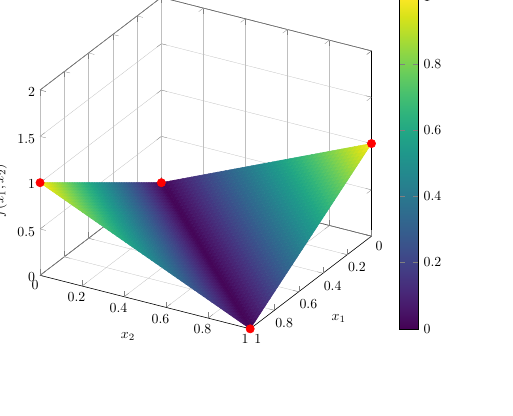
\begin{tikzpicture}[scale=0.5]
  \begin{axis}[
      width=10cm,
      height=10cm,
      xlabel={$x_1$},
      ylabel={$x_2$},
      zlabel={$f(x_1, x_2)$},
      zmin=0, zmax=2,
      domain=0:1,
      samples=50,
      mesh/ordering=y varies,
      view={120}{30},
      grid=major, % Adding grid lines
        major grid style={line width=.2pt,draw=gray!50},
        % minor grid style={line width=.1pt,draw=gray!20},
        xtick={0,0.2,0.4,0.6,0.8,1},
        ytick={0,0.2,0.4,0.6,0.8,1},
      colorbar,
      colormap/viridis
  ]

  % Define the piecewise function for the Lovász extension
  \addplot3[
      surf,
      mesh/interior colormap name=viridis,
      shader=flat,
      z buffer=sort,
  ] 
  (x, y, 
      {x <= y ? (y-x) : (x-y)}
  );

  % Draw the original points and their function values
  \addplot3[only marks, mark=*, mark options={color=red, scale=1.5}] coordinates {
      (0,0,0) % f(emptyset) = 0
      (1,0,1) % f({1}) = 1
      (0,1,1) % f({2}) = 2
      (1,1,0) % f({1, 2}) = 2
  };
  
  \end{axis}
\end{tikzpicture}
\caption{Lovász extension of a set-function $F$}
\efig

\end{example}

\begin{example}
  Let consider a set-function, $F : 2^{\{1, 2\}} \to \R$
  such that, $F(\varnothing) = 0, F(\{1\}) = 1, F(\{2\}) = 1, F(\{1, 2\}) = 3$.
  
  The Lovász extension of the above function is as follows:
  \bd
  f([x_1; x_2]) = \begin{cases}
    x_1 + 2x_2 & \text{ if }x_1 \geq x_2\\
    2x_1 + x_2 & \text{Otherwise}
  \end{cases}
  \ed
  \bfig[h!]
  \centering
  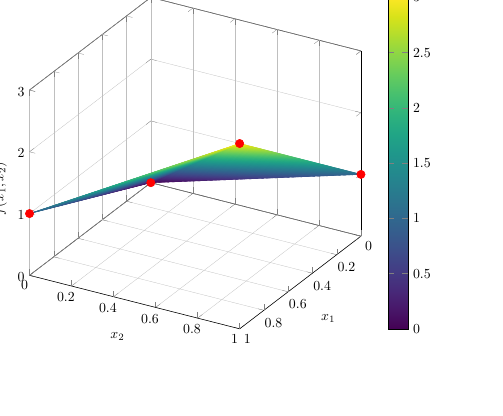
\begin{tikzpicture}[scale=0.5]
    \begin{axis}[
        width=10cm,
        height=10cm,
        xlabel={$x_1$},
        ylabel={$x_2$},
        zlabel={$f(x_1, x_2)$},
        zmin=0, zmax=3,
        domain=0:1,
        samples=50,
        mesh/ordering=y varies,
        view={120}{30},
        grid=major, % Adding grid lines
        major grid style={line width=.2pt,draw=gray!50},
        % minor grid style={line width=.1pt,draw=gray!20},
        colorbar,
        colormap/viridis
    ]
  
    % Define the piecewise function for the Lovász extension
    \addplot3[
        surf,
        mesh/interior colormap name=viridis,
        shader=flat,
        z buffer=sort,
    ] 
    (x, y, 
    {x <= y ? 2 * x + y : 2 * y + x} 
    );
  
    % Draw the original points and their function values
    \addplot3[only marks, mark=*, mark options={color=red, scale=1.5}] coordinates {
        (0,0,0) % f(emptyset) = 0
        (1,0,1) % f({1}) = 1
        (0,1,1) % f({2}) = 2
        (1,1,3) % f({1, 2}) = 2
    };
    \end{axis}
  \end{tikzpicture}
  \caption{Lovász extension of a set-function $F$}
  \efig

  \end{example}



\begin{proposition}
Let $F$ be any set-function, we have:
\begin{enumerate}
  \item If $F$ and $G$ are set-functions with Lovász extensions $f$ and $g$ respectively, then
  $f + g$ is the Lovász extension of $F + G$.
  \item For $\w \in \R_+^{p}, f(\w) = \int_{0}^{\infty}F(\{\w \geq z\})dz$.
  \item If $F(\V) = 0 \implies \forall \w \in \R^{p}, f(\w) = \int_{-\infty}^{\infty}F(\{\w \geq z\})dz$.
  \item For all $\w \in \R^p$ and $\alpha \in \R$, $f(\w + \alpha 1_{\V}) = f(\w) + \alpha F(\V)$.
  \item The Lovász extension $f$ is positively homogeneous with degree-1.
  \item For all $\A \subseteq \V, F(\A) = f(1_{\A})$.
  \item If $F$ is symmetric (i.e, $\forall \A \subseteq \V, F(\A) = F(\V \backslash \A)$), then $f$ is even.
  \item If $\V = \A_1 \cup \dots \A_m$ is a partition of $\V$, and $\w = \sum_{i=1}^{m}\nu_i 1_{\A_i}$ with
  $\nu_1 \geq \nu_2 \geq \dots \nu_m$ then $f(\w) = \sum_{i=1}^{m-1}(\nu_i - \nu_{i+1})F(\A_1 \cup \dots \cup \A_i) + \nu_mF(\V)$.
  \item If $\w \in [0, 1]^p$, then $f(\w) = \mathbb{E}_{x \sim Uniform([0, 1])}\left[F(\{\w \geq x\})\right]$.
\end{enumerate}
\end{proposition}

\begin{proposition}
A set-function $F$ is submodular if and only if its Lovász extension $f$ is convex.
\end{proposition}


\begin{proposition}
Let $F$ be a submodular function and $f$ be its Lovász extension. 
Then $\min_{\A \subseteq \V}F(\A) = \min_{\w \in \{0, 1\}^{p}}f(\w) = \min_{\w \in [0, 1]^{p}}f(\w)$
\end{proposition}

\section{Submodular Optimization}
\textbf{A few properties:} Let $F: 2^{\V} \to \R$ be a submodular function, then
\begin{enumerate}
\item \textbf{Optimality Conditions:} If $\A \subseteq \V$ is a minimizer of $F$ if and only if $\A$ is minimizer of $F$ overall
subsets of $\A$ and all supersets of $\A$.
\item \textbf{Lattice of Minimizers:} If $\A$ and $\B$ are minimizers of $F$, then so are $\A \cup \B$ and $\A \cap \B$.
\item \textbf{Minimizing a Submodular Function:} 
\begin{theorem}[Grötschel-Lovász-Schrijver '81]
  There is an algorithm that computes the minimum of any submodular
  function $F: 2^{\V} \to \R$ in $poly(|\V|)$ time.
\end{theorem}
\item Maximizing a submodular function is \textbf{NP-Hard} in general.\\
\textbf{Greedy Algorithm:} Pick elements one-by-one, maximizing the gain
in $F(\S)$, while maintaining $\S \subseteq \V$ i.e, $\S \gets \S \cup \argmax_{i \in \S}F(\S \cup \{i\}) - F(\S)$.
\begin{theorem}[Nemhauser, Wolsey, Fisher ’78]
If $F$ is non-decreasing submodular Greedy Algorithm finds a solution
of value atleast $(1-1/e) \times$ Optimal value for the problem $\max\{F(\S): |\S| \leq k\}$.
\end{theorem}
\begin{theorem}[Nemhauser, Wolsey ’78]
No algorithm using a polynomial number of
queries to $F$ can achieve a factor better than $(1-1/e)$.
\end{theorem}

\end{enumerate}

\subsection{Structured Sparsity}
Consider the following regression problem with structured sparsity inducing norm,
We can also consider the following optimization problem,
\bd
\min_{\w \in \R^{p}}\frac{1}{N}\sum_{i=1}^{N}\mathcal{L}(\y_i, \IP{\w}{\x_i}) + \lambda' F(S(\w))
\ed
where, here, $S$ is the support of $\w$, $F$ is set-function penalizes discretely over the support set 
(it is submodular). The above problem
is a combinatorial optimization problem, and is computationally intensive. We can relax the above to below problem,
\bd
\min_{\w \in \R^p}\frac{1}{N}\sum_{i=1}^{N}\mathcal{L}(\y_i, \IP{\w}{\x_i}) + \lambda \Omega_{S}(\w)
\ed
where, $\Omega_{S}$ is a gauge function, and $\lambda$ is a regularization parameter. The above problem is a convex optimization problem.

We ideally want a optimal convex relaxation of the original problem. The below proposition gives us a way to do that.
\begin{proposition}
Let $F$ be a non-decreasing submodular function. The function $\Omega_{S}: \w \to f(|\w|)$ is the tightest convex lower
bound (dual of dual) of the function $\w \to F(S(\w))$ on the unit $L_{\infty}$ ball, $[-1, 1]^p$, here $f$ is 
the Lovász extension of $F$.
\end{proposition}

\textbf{LASSO:} The Lovász extension of the cardinality function, $F(\A) := |\A|$ is $f(\w) = \IP{\w}{1_{\V}}$.
Therefore, the tightest convex lower bound of $L_0$ norm is $L_1$ norm.



Let consider a set-function, $F : 2^{\{1, 2\}} \to \R$
such that, $F(\varnothing) = 0, F(\{1\}) = 1, F(\{2\}) = 1, F(\{1, 2\}) = 2$.
  
We have that $f([|x_1|; |x_2|])$
\bd
f([x_1; x_2]) = |x_1| + |x_2|
\ed
\bfig[h!]
\centering
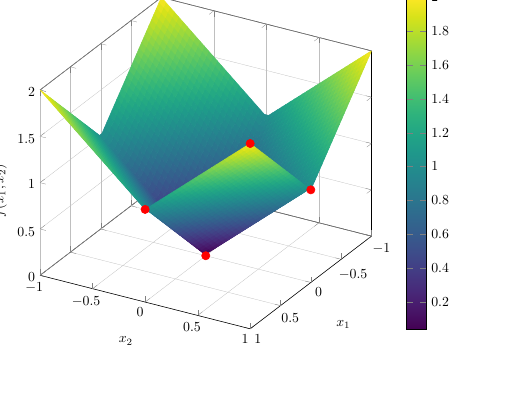
\begin{tikzpicture}[scale=0.5]
  \begin{axis}[
      width=10cm,
      height=10cm,
      xlabel={$x_1$},
      ylabel={$x_2$},
      zlabel={$f(x_1, x_2)$},
      zmin=0, zmax=2,
      domain=-1:1,
      samples=50,
      mesh/ordering=y varies,
      view={120}{30},
      grid=major, % Adding grid lines
      major grid style={line width=.2pt,draw=gray!50},
      % minor grid style={line width=.1pt,draw=gray!20},
      colorbar,
      colormap/viridis
  ]

  % Define the piecewise function for the Lovász extension
  \addplot3[
      surf,
      mesh/interior colormap name=viridis,
      shader=flat,
      z buffer=sort,
  ] 
  (x, y, 
      {abs(x) + abs(y)}
  );

  % Draw the original points and their function values
  \addplot3[only marks, mark=*, mark options={color=red, scale=1.5}] coordinates {
      (0,0,0) % f(emptyset) = 0
      (1,0,1) % f({1}) = 1
      (0,1,1) % f({2}) = 2
      (1,1,2) % f({1, 2}) = 2
  };
  \end{axis}
\end{tikzpicture}
\caption{Lovász extension of a set-function $F$}
\efig



\bibliographystyle{plain}
\bibliography{refs}

\end{document}
